\subsection{Development Board}
In order to prototype our sensor node software, LoRaWAN gateway, and server, we are using a development board that uses the same microcontroller and LoRa module that we are going to use for our final design. That development board is the Seeed LoRa-E5 mini. The development board itself is fairly barebones, containing only the LoRa module itself (the STM32WLE5JC), some I/O pins, a USB Type-C input for power, and some antenna connectors. The board does not contain a USB-based programmer, only SWD pins. Instead we had to purchase an external STLink programmer to be able to connect the development board to our computer for programming. An image of the development board can found in Figure \ref{fig:dev-board}.

\begin{figure}
    \centering
    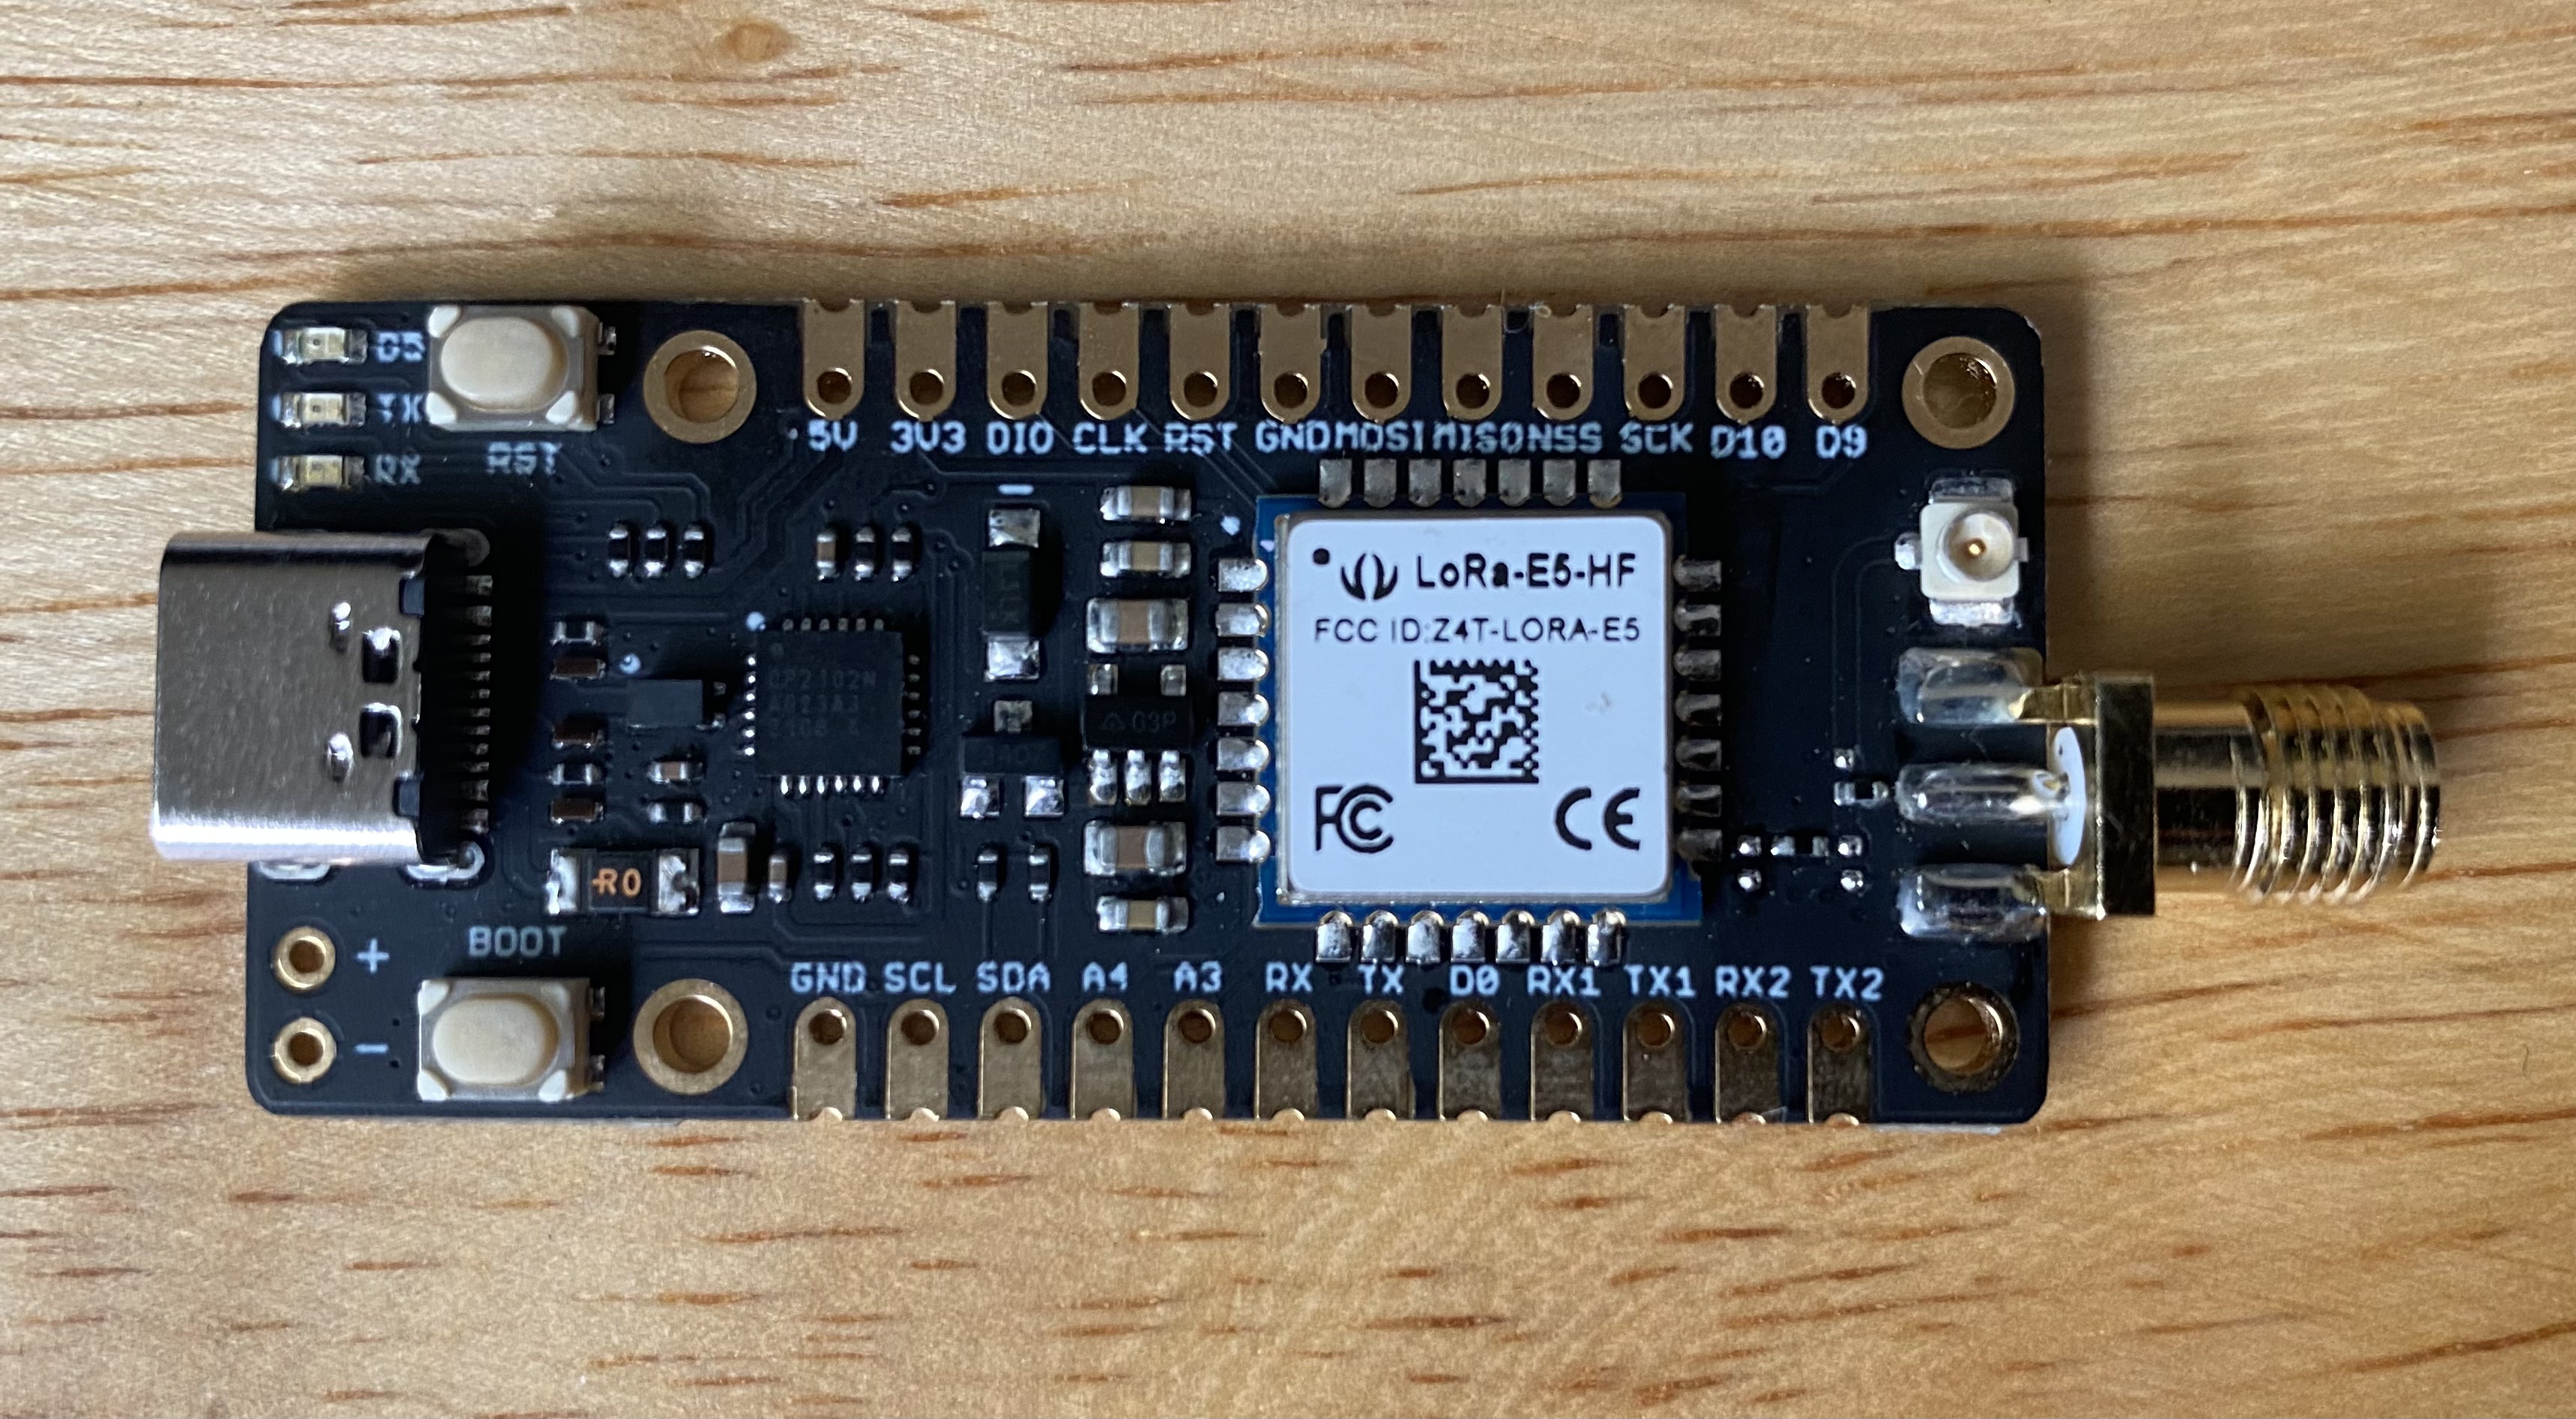
\includegraphics[width=4in]{figures/dev-board.png}
    \caption{The LoRa-E5 mini development board that we are using to prototype our software}
    \label{fig:dev-board}
\end{figure}